\section{Model-Based RL}\label{sec:model-based}
In the previous section, Actor-Critic methods were implemented on both the CartPole and Catch environments. The inclusion of an inductive bias exploiting the symmetry of an MDP led to improvements in the sample efficiency of learning an expert policy, while maintaining robustness to initialization conditions.
In the case where the transition dynamics of the MDP are group-structured, or approximately group-structured, this report proposes the use of an equivariant world model. With a world model that has inductive biases designed to aid in learning the MDP's transition dynamics, the world model may be learned more efficiently and accurately from fewer samples from the environment, improving the effectiveness of planning for the agent.

The specific algorithm implemented to create a model-based agent is a dyna~\ref{sec:Dyna} algorithm, with a PPO \ref{sec:PPO} agent. Using the dyna-PPO agent means that when the number of planning steps is set to zero, the agent becomes a model-free PPO agent, enabling direct comparison with the baseline MLP PPO implementation~\ref{sec:baseline}.

Both Catch and CartPole are environments where the reward function is only a function of the state the agent is in, and not a state-action pair. Further, because their rewards are simple functions of their state, this report forgoes learning the reward dynamics of the environments and uses their existing reward structure on simulated states, such that:
\begin{equation}
	R_{t+1} = R(T(s, a)).
\end{equation}
Where, $R$, is the reward function defined by the environment.

\subsection{Constructing Transition Models}
Before using a full model-free algorithm, where the model is learned online, during the training. A simplified algorithm, supervised-dyna, is tested that uses offline trained world models. The process for this is outlined below:
\begin{algorithm}
	\caption{Supervised-Dyna}\label{alg:Supervised-Dyna}
	\begin{algorithmic}
		\State Initialize $T_\phi$
		\State Sample transition tuples from a policy $\pi \sim (s, a, s')$ on MDP $\mathcal{M}$.
		\Comment {Here $\pi$ is a random/ expert policy}
		\State Form Dataset $\mathcal{D}$ from sampled transition tuples.
		\For {Num Epochs}
		\State $\phi' \leftarrow $Minimise $L(\phi , \mathcal{D})$.
		\EndFor
		\For {Num Dyna Iterations}
		\For {Num Acting Updates}
		\State Sample transition tuples from policy $\pi_\theta \sim (s, a, s')$ on $\mathcal{M}$
		\State Train agent $\pi_\theta$ from direct samples.
		\EndFor
		\For{Num Planning Updates}
		\State Sample transition tuples from policy $\pi_\theta \sim (s, a, s')$ on $T_\phi$.
		\State Train agent $\pi_\theta$ from planned samples.
		\EndFor
		\EndFor
	\end{algorithmic}
\end{algorithm}

Using offline-trained world models has benefits as an intermediate step. Firstly, the world model is stationary throughout the agent training process and can be easily investigated. Secondly, the model can be trained with ample data. This is in contrast to full dyna where the length of the planning and acting phases must be tuned as a hyperparameter, and the convergence of the models must be tuned. This hyperparameter of $\text{Num Acting Updates}/\text{Num Planning Updates}$, is referred to as the Planning ratio.


\subsection{Proximal Pooling Motivation}
To produce equivariant world models, there are additional challenges beyond just implementing a G-CNN, which permutes its outputs depending on the input transformation. In contrast to an equivariant actor, where simply permuting the logits of a distribution suffices for equivariant behaviour \ref{symmetrizer}, building an equivariant world model with a G-CNN means the output of the network predicts not only the next state but also a number of nonsense next states.

To illustrate what the final layer output in the G-CNN is doing, consider the same setup as in the Actor-Critic networks, where there is a hidden representation whose responses get permuted depending on the application of a group-structured transformation on the input:

\begin{equation}
	f(s , a) = \begin{pmatrix}
		g(s, a)                                     \\
		g(\ell_1^\mathcal{S}s,\ell^\mathcal{A}_1a)  \\
		g(\ell^\mathcal{S}_2s, \ell^\mathcal{A}_2a) \\
		\vdots                                      \\
		g(\ell_{|G|}^\mathcal{S}s, \ell^\mathcal{A}_{|G|}a),
	\end{pmatrix}
\end{equation}
and when a transformation is applied to the input these responses, $g$ are permuted,
\begin{equation}\label{eq:tm_gcnn}
	f(\ell_i^\mathcal{S}s, \ell_i^\mathcal{A}a) = \mat{P}_i f(s, a).
\end{equation}
Because the permutations are defined by the group, these are the same permutations as in Eq.\ref{eq:gs_perm}. However, here each response $g: \mathcal{S} \times \mathcal{A} \rightarrow \mathcal{S}$, produces a transition image. In order to obtain a transition function there must be a method to pool over the responses.

\subsection{Group Action Transformation}
When the network $f$ performs a forward pass and outputs the vector of responses, as described by Eq.\ref{eq:tm_gcnn}, the equivariance in the response maps group actions on a state space to a permutation of responses that all have the same shape as the state. This is not the equivariance constraint that is required for a transition model, which is:
\begin{equation}
	T(\ell_i^\mathcal{S}s, \ell_i^\mathcal{A}a) = \ell_i^\mathcal{S}T(s, a).
\end{equation}
The first step in achieving this is to apply a group action to each row of the response of $f$. This is the Action Transformation operation, denoted as $\mat{\mathcal{T}}$, where,
\begin{equation}
	\mat{\mathcal{T}}f(s,a) = \begin{pmatrix}
		g(s, a)                                                          \\
		\ell_{-1}^\mathcal{S}g(\ell_1^\mathcal{S}s,\ell^\mathcal{A}_1a)  \\
		\ell_{-2}^\mathcal{S}g(\ell^\mathcal{S}_2s, \ell^\mathcal{A}_2a) \\
		\vdots                                                           \\
		\ell_{-|G|}^\mathcal{S}g(\ell_{|G|}^\mathcal{S}s, \ell^\mathcal{A}_{|G|}a)
	\end{pmatrix}.
\end{equation}
Due to group closure, this gets us quite close to equivariance! For example consider some group element, which is the inverse of $i$ acting on the input,

\begin{equation}\label{eq:g-cnn}
	\mat{\mathcal{T}}f(\ell_{-i}^\mathcal{S}s,\ell_{-i}^\mathcal{A}a) = \begin{pmatrix}
		g(\ell_{-i}^\mathcal{S}s,\ell_{-i}^\mathcal{A}a)                 \\
		\ell_{-1}^\mathcal{S}g(\ell_j^\mathcal{S}s,\ell^\mathcal{A}_ja)  \\
		\ell_{-2}^\mathcal{S}g(\ell^\mathcal{S}_ks, \ell^\mathcal{A}_ka) \\
		\vdots                                                           \\
		\ell_{-i}^\mathcal{S}g(s, a)                                     \\
		\vdots                                                           \\
		\ell_{-|G|}^\mathcal{S}g(\ell_{|G|}^\mathcal{S}s, \ell^\mathcal{A}_{|G|}a)
	\end{pmatrix}.
\end{equation}
Then, to achieve equivariance, the correct row must be selected. This would be straightforward if the group action on the input were known, but in general, it is not. However, in many cases, in a transition model, the output is closer to the input than to any of the other states. With this proximity intuition, a pooling method is introduced to gain approximate equivariance with the transition models. This vector of next states is referred to as transition images.
When using CNNs or other G-CNNs for classification or other image processing tasks, a reduction pooling method such as mean or max is used over the different groups. Both of these pooling types result in an invariant network. Specifically, if one pools over the group, taking either a mean or a max over the group dimension of $f$, the output remains unchanged when the group dimension is permuted, because the transformation applies only a permutation along this axis
\begin{equation}
	\max_\text{axis G} \mat{P}_i f(s, a) = \max_\text{axis G} \mat{P}_j f(s, a), \forall i, j.
\end{equation}
Here the group axis, axis G, is the leading dimension in $f$ if $f: \mathcal{S} \times \mathcal{A} \rightarrow \mathbb{R}^{|G| \times \mathcal{S}}$. This invariance is not helpful in our case and so an alternative technique of pooling over possible next states is proposed.


\subsection{Proximal Pooling Layers}\label{sec:proximal_pool}
As a caveat, this method does not guarantee equivariance to the input transformation. However, empirically, it is effective. The proximal pooling layer, $\mathcal{P}$, takes a distance metric, $d(s, s')$, and selects the transition image, which has the minimum distance metric as such the full approximately equivariant network is;
\begin{equation}
	T(s, a) = \mathcal{P}\mathcal{T}f(s, a)  =\arg \min_\text{axis G} d \left (s,  \begin{pmatrix}
			g(s, a)                                                          \\
			\ell_{-1}^\mathcal{S}g(\ell_j^\mathcal{S}s,\ell^\mathcal{A}_ja)  \\
			\ell_{-2}^\mathcal{S}g(\ell^\mathcal{S}_ks, \ell^\mathcal{A}_ka) \\
			\vdots                                                           \\
			\ell_{-|G|}^\mathcal{S}g(\ell_{|G|}^\mathcal{S}s, \ell^\mathcal{A}_{|G|}a)
		\end{pmatrix}
	\right ).
\end{equation}
The $\arg \min_\text{axis G}$, returns the state image, which is closest to the original state, if the network predictions are better than random with respect to the distance metric.

Empirically, across 10,000 randomly sampled CartPole states, the network, $T(s, a)= \mathcal{P}\mathcal{T}f(s,a)$, is fully equivariant, when untrained. When trained, it is equivariant across the same sample, and also achieves better validation MSE than the non-equivariant model, when trained on transitions from the same data.

This is not the case for the Catch network. Catch has $675$ state-action pairs, and the transition model when untrained achieves $98.3 \pm 0.6\%$ equivariance across all these state action pairs. The standard error is quoted over 1,000 random seed parameter initializations. The performance of the transition models is investigated in more depth in sections\ref{something,something}.

When trained, the Catch model is able to achieve a validation accuracy of 1. As such, the lack of perfect equivariance may not be an issue in some scenarios. Small, discrete spaces with a high degree of symmetry are the worst in terms of a lack of equivariant predictions, as the expected distance between any two states decreases. Additionally, for MDPs where no sensible distance metric can be constructed, this method will fail.

\begin{proposition}
	Given some distance metric between two states $d(s, s')$ and a G-CNN transition model of the form Eq.\ref{eq:g-cnn}. If at some time $t$ a state transition from $s_t$ to $s_{t+1}$ takes place. And the MDP has a group structured discrete symmetry, if the state space obeys,
	\begin{equation}
		d(s_t, s_{t+1}) < \mathbb{E}_{s'\sim \mu}[d(s_t, s')], \forall i, s_t.
	\end{equation}
	Where $\mu$ is the steady state distribution. Then, a proximal pooling layer can be used to make the G-CNNs' forward pass approximately equivariant.
\end{proposition}
As motivation for why this occurs, when the G-CNN performs a forward pass, one of the multiple outputs of $\mathcal{T} f(\ell_i^\mathcal{S}s,\ell_i^\mathcal{A} a)$, is empirically non correlated to the other group members, for all parts of the state affected by the transformations.
\begin{figure}[h!]
	\centering
	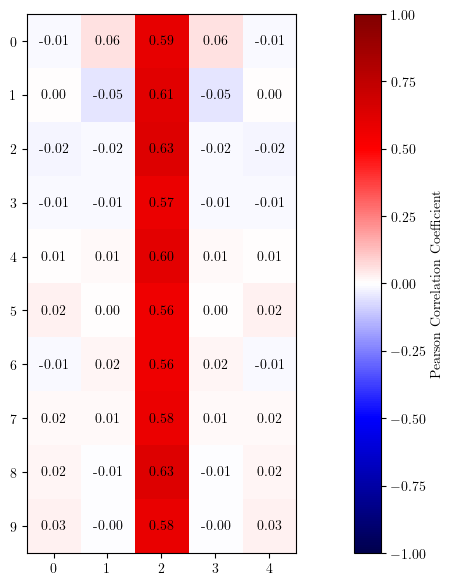
\includegraphics[width = 0.6\textwidth]{Figures/logits_correlation.png}
	\caption{Pearson $r^2$ value for each logit in the output of the transition model between $g(s, a)$ and $\ell_r^\mathcal{S}g(\ell_r^\mathcal{S}s,\ell_r^\mathcal{A}a)$, for one of the 675 possible state action pairs, across 1000 random  seeds for network initialization. }
	\label{fig:logits_correlation}
\end{figure}
Empirically, one can see the lack of correlation in Fig.\ref{fig:logits_correlation}, which plots the $r^2$ co-efficient between the transition images across 1,000 randomly initialized untrained networks. The network parameterizes the next states as two distributions, by outputting an array of 50 logits. As expected, the network responses along the centre axis should be invariant to the input transformation. Thus, a positive correlation coefficient is encouraging. For all other logits in the distribution over the next state there is no evidence of a correlation between the two transition images, at a 5\% significance level.

With the two outputs being independent of each other, the correct next state can be selected using the proximal layer reliably, and the networks can be approximately equivariant.



\subsection{CartPole}
A CartPole transition model is a functional approximation to a deterministic, non-linear system.
To learn this transition model, transitions are sampled from a policy on the MDP and stored. This is then used as a dataset to perform supervised learning on. The Transition model, $T_\phi: \mathcal{S} \times \mathcal{A} \rightarrow \mathcal{S}$, predicts next states from a state action-pair.

The loss function for the transition model is the average L2 distance between the predicted next state and the true next state across a batch of samples.
\begin{equation}
	L(\phi) = \frac{1}{N}\sum^N_{(s, a, s')_i \sim \mathcal \tau} (1-\delta(\text{done}))||T(s, a) - s'||_2
\end{equation}
Here $\tau = \{(s, a , s')_1^N\}$ is a batch of transitions, of size $N$, sampled from the MDP, and $(s, a, s')$, is the state, action, next state tuple. Often, a reward model is required to also simulate an MDP. For simplicity, the CartPole reward model is used, rather than learned. The one subtlety is that the loss is only back-propagated if $s$, is not a terminal state. The indicator function $\delta(\text{done}) = 1 \text{if $s$ is terminal} $. Thus, the model only learns transitions governed by the environment dynamics and not how to reset the episode.


\subsubsection{Constructing Equivariant World Models}
Like in the previous section on \ref{sec:actor-critic}, the equivariant transition models are deep G-CNNs. In contrast to equivariant Actors in the previous section, these networks have to use the proximal pooling layer on their output \ref{sec:proximal_pool}. The equivariance described by these networks is to the identity and negative operation, such that;
\begin{equation}
	T(- s, 2*a - 1) =  -T(s, a), \forall
\end{equation}
These transition models are not truly equivariant but empirically, the proximal pooling layer suffices to meet the equivariance condition. As a distance metric to achieve the equivariance, the proximal pool uses the $L1$ distance.

Similarly to the actor networks, the transition models have two hidden Group Convolution layers. The input layer for actions also transforms the action from $[0, 1]$ to $[-1, 1]$. Thus, the same group convolution layer can be used for both the state and the action input.


\subsubsection{Results: Comparing Convergence of Transition Models}
In order to perform model based RL, a transition model must be learnt to simulate transitions, such that the agent can learn a policy that performs better in the original environment. Thus, the first set of experiments was supervised training of transition models.

Three different pairs of models were trained. The first pair was trained on data collected from an expert and random policy(joint expert-random), where half of the data is sampled from an expert policy, and half from a random policy. The second pair took the first dataset and filtered out the transitions that took the right action (left-hand). The final pair was trained only on data sampled from a random policy (random).
\begin{figure}
	\centering
	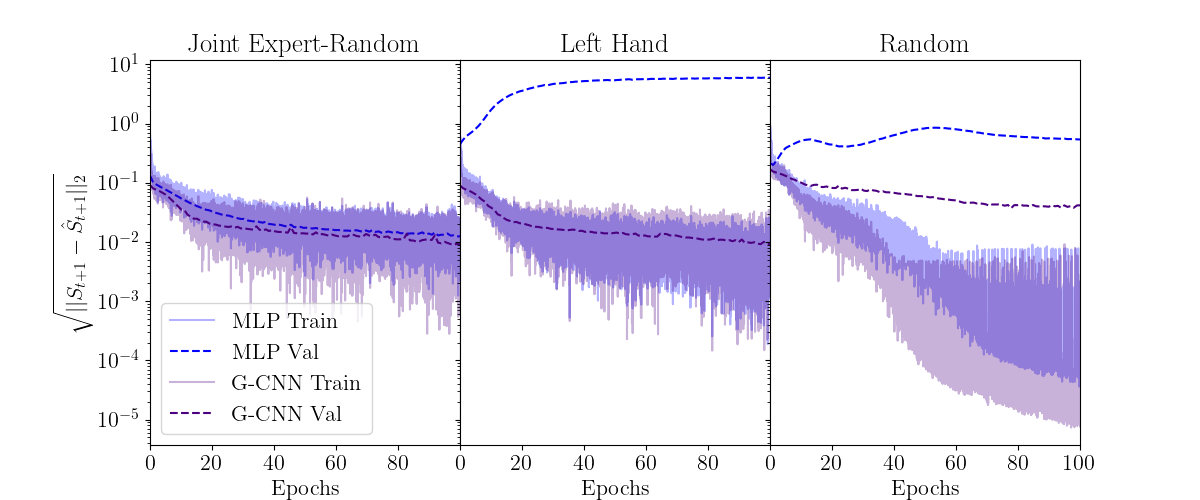
\includegraphics[width=\linewidth]{Figures/transition_model_loss.png}
	\caption{Transition Model RMS error, plotted against epochs for three different training datasets. Left, the joint expert-random dataset. Center, the same dataset as left, however, with only the left action taken. Right, solely transitions sampled from a random policy. These datasets contain 40,000 transitions. All plots have the same set of validation data with a 50/50 split of expert and random policy sampled data.}
	\label{fig:transition_model_cp}
\end{figure}

In Fig.\ref{fig:cartpole_equivariant_actor} it is clear that the G-CNN, despite having the same parameter count, performs better on all three transition datasets. On the joint expert-random dataset, the final delta in validation root-mean-square (RMS) is $\approx 0.003$.

Further, when the right action is filtered out, there was a reassuringly stark delta in performance between the equivariant model and the conventional MLP transition model. As expected, the equivariant model recovered the majority of the performance in this scenario, recovering slightly better RMS error, $0.0093$ and $0.0091$ for the joint expert-random and left-hand datasets respectively. This may not be a significant delta. The MLP, on the other hand, appears to overfit to left actions heavily. Then when the MLP is asked to generalize to transitions that it has not seen it fails.

Interestingly, when only random data is sampled, the equivariant model has lower validation loss. To further investigate these trends, the final transition model validation loss is plotted by angle for each of the datasets in Fig.\ref{fig:cp_model_angle}.


\begin{figure}[h!]
	\centering
	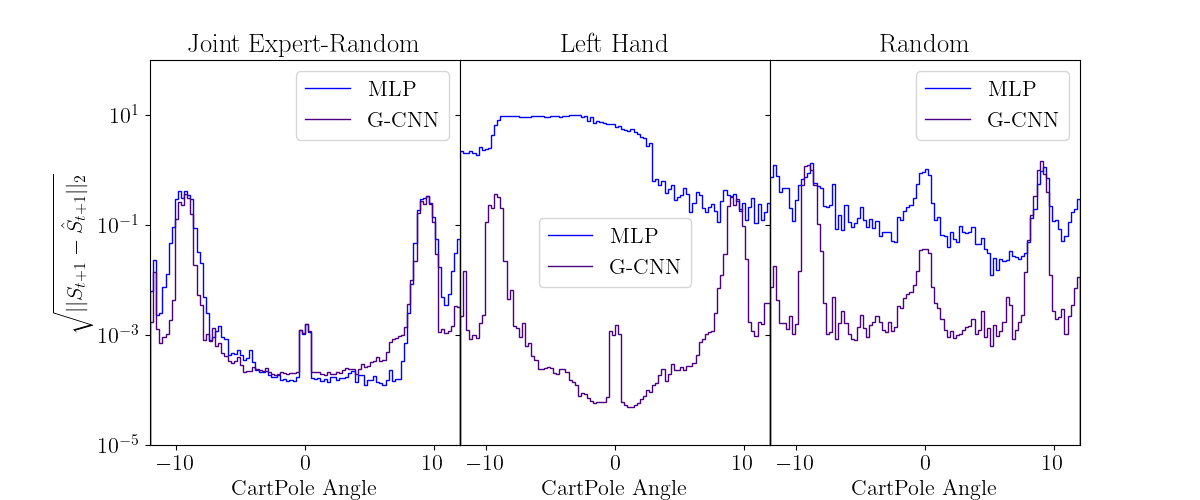
\includegraphics[width=0.95\textwidth]{./Figures/cart_pole_by_angle.png}
	\caption{RMS Error plotted by angle on validation transitions sampled from a 50/50 split of expert and random data. Left, models trained on a dataset of 50/50 sampled expert and random policy transitions. Center, only transitions taking the left action. Right, transitions only sampled from a random policy.}
	\label{fig:cp_model_angle}
\end{figure}

In the figure on the left, the RMS error is substantially lower for the equivariant model, for $\theta <|5^o|$. This indicates that the equivariant constraints and the structure of the model improves the accuracy of the model in comparison to the MLP, especially in the region where CartPole's dynamics are linear due to the limited moments applied by the pole. This trend is seen across all datasets. For all transition models there is a sharp increase in RMS error around $8^o$. The RMS error then falls as the pole deviates further from horizontal. Currently, this is a topic for further investigation.

The Centre plot in Fig.\ref{fig:cp_model_angle}, is as expected. The RMS errors were similar for the equivariant G-CNN, and the MLP performs slightly better on a pole leaning to the right.

In the last plot, where the model is trained solely on transitions sampled from random actions, a striking result is obtained. The equivariant model performs notably better across all angels, with an RMS validation error of $0.039$, in comparison of that to the MLP of $0.19$. On validation data that is sampled jointly from an expert policy, where the majority of transitions are at small angles.

This superior generalization is demonstrated when the model is trianed on random data but validated on join expert random data, which contains far more transitions at small angles.

This property may be important in training dyna Agents. Where initially the agents' policies are suboptimal and may tend to be worse at keeping the pole upright. However, the agents' learning in the simulated environments may be augmented by the improved generalization to small angels. As the policies improve from simulated experience, they tend towards having more transitions at small angels.\footnote{The transition distributions can be found in the Appendix.\ref{ap:dist_cp}.}

\subsubsection{Results: Supervised-Dyna}
Using the off-line trained world models above on the joint expert-random data. Both actor-critic agent were trained using the supervised-dyna algorithm~\ref{alg:supervised-dyna}. The model-based agents have 50 dyna iterations, and the full hyperparameter set can be found in the appendix~\ref{ap:supervised-dyna-catch-hyp}. Further, a hyperparameter sweep was performed over planning ratio and the best planning ratios were chosen.
\begin{figure}\label{fig:supervised-dyna-cp}
	\centering
	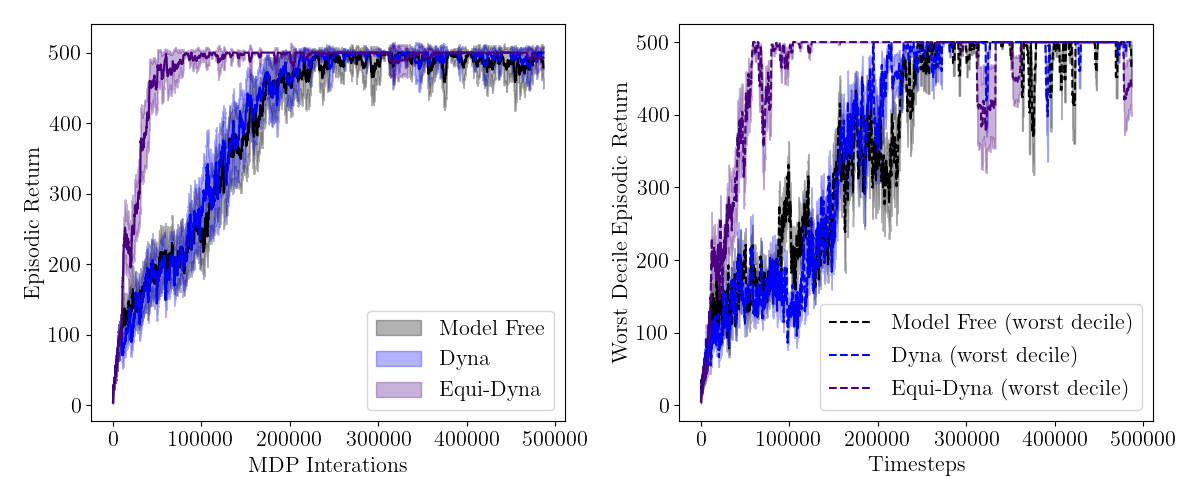
\includegraphics[width=\textwidth]{Figures/Expert_dyna_cp_best.png}
	\caption{Left: Mean episodic returns for the CartPole agents across 128 random seeds
		plotted against number of interaction time-steps in the MDP. Right: The mean
		cumulative episodic returns of the worst performing 128 random seeds against
		number of experience time-steps in the MDP. Both of the plots are moving
		averages, with windows of 10 time-steps. Additionally, two standard errors are
		plotted. The equi-dyna model uses a planning ratio of 8 and the Dyna model uses a planning ratio of 1.}
\end{figure}
The results are displayed in Fig.\ref{fig:supervised-dyna-cp}. Where the equi-dyna model was found to perform best with a high planning ratio. The small difference in validation loss between the transition models appears to have a large impact on the quality of the planning available to the agents, with the dyna model only providing a small uplift over a model-free baseline.
\begin{table}
	\centering
	\begin{tabular}{|c|c|c|c|}
		\hline
		Time-steps & Baseline     & Dyna                 & Equi-Dyna             \\
		\hline
		$10, 000$  & $102 \pm 5$  & $110 \pm 10$         & $\mathbf{120 \pm 10}$ \\
		$100, 000$ & $260 \pm 10$ & $245 \pm$ 20         & $\mathbf{498 \pm 2}$  \\
		$500,000$  & $497 \pm 1$  & $\mathbf{500 \pm 1}$ & $498 \pm 13$          \\
		\hline
	\end{tabular}
	\caption{Cumulative episodic returns tabulated for the three network architectures. All episodic returns are recorded with confidence intervals of two standard errors across 128 random seeds.}
	\label{tab:supervised-dyna-cp}
\end{table}

This trend, when investigated at the $20\%, 40\%$, and $100\%$ completion in Table.\ref{tab:supervised-dyna-cp} is clear. Particularly impressively, at $40\%$ of the sampled experience the equi-dyna model is able to achieve an expert policy on average. With further training, it seems that the policy diverges further. This is the most sample efficient model yet, and suggests that with a sufficiently good world model, the agent may be able to achieve strong generalization performance.
\subsection{Catch}

Again construction of the G-CNN is much the same as in the case for CartPole. The basic network was built from group convolutions, with two hidden layers. There is one notable difference between these models and the CartPole models. The output for the Catch transition models are two distributions over the ball and paddle locations. In contrast to the real valued outputs of the CartPole model. These distributions are $T(s, a)_b, T(s, a)_p$ which are the distribution over the ball and paddle locations, respectively.
\begin{equation}
	L(\phi) = \frac{1}{N}\sum_{(s, a, s') \sim \tau}^N(1- \delta (\text{done}))\left[BCE(s', T(s, a)_b) + BCE(s', T(s, a)_p)\right] .
\end{equation}
Where $BCE$ is the binary cross entropy between two distributions. The same indicator function is used to ensure that the model only learns from non-terminal states.

In order to make the model equivariant the proximal pooling layer requires  a distance metric. This needs to quantify how far apart the predictions are. The metric used was an L1 loss between the x, y position in $s$ and $T(s,a)$ of both the ball and the paddle. Additionally, to make the possible number of distances greater when the distances are summed, the ball's displacement is multiplied by 0.13. This constant value was found to improve the equivariance behaviour of the proximal pooling layer. The distance metric is then given by,
\begin{equation}
	d(s, s') = ||\text{mode}(T(s, a)_b) - s'_b||_1 + 0.13 ||\text{mode}(T(s, a)_p )- s'_p||_1.
\end{equation}
The subscripts, $b, p$ indicate the ball and the paddle, respectively.

\subsubsection{Results: Comparing Convergence of Transition Models}
As before for CartPole, the transition models were trained on three different datasets to assess their convergence behaviour. Again the datasets were a random and expert policy sampled data, only left actions from the previous dataset, and only random policy sampled transitions.

\begin{figure}
	\centering
	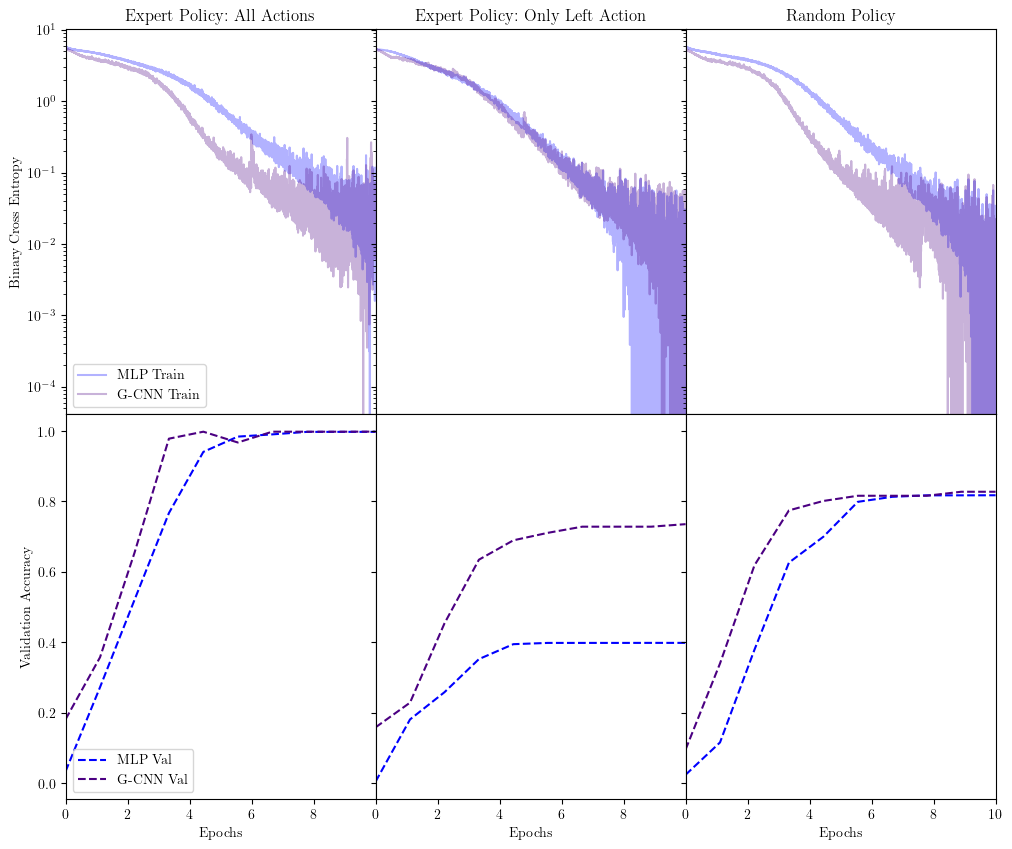
\includegraphics[width=\linewidth]{Figures/transition_model_catch.png}
	\caption{Transition Model BCE error, plotted against epochs for three different training datasets, With model validation accuracy plotted below. Left, the dataset is joint expert-random. Center, the same dataset as left, however, with only the left action taken. Right, solely transitions sampled from a random policy. These datasets contain 400,000 transitions. All plots have the same set of validation data with a 50/50 split of expert and random policy sampled data.}
	\label{fig:transition_model_catch}
\end{figure}

In Fig.\ref{fig:transition_model_catch}, the equivariant model again demonstrates the benefits of inductive biases. The equivariant and MLP models achieve $0.998$ validation accuracy on transitions sampled from the joint expert random policy, with slightly faster convergence. When the model acts on a dataset, which has been filtered for only the left actions. The equivariant G-CNN generalizes to both actions as expected. The Equivariant model preforms slightly better on the random data. However, the performance is lack luster. On inspection the random dataset contains $60$ of the unique transitions found in the join expert-random dataset. This implies that both models are struggling to generalize.

\subsubsection{Results: Supervised-Dyna}
Again, three agents were trained over 128 random seeds. To compare the performance the equivariant G-CNN dyna against an MLP transition model with a baseline actor-critic. The number of dyna iterations was set to 50 for both the MLP transition model dyna agent (dyna) and the equivariant transition model (equi-dyna) agent.

\begin{figure}
	\centering
	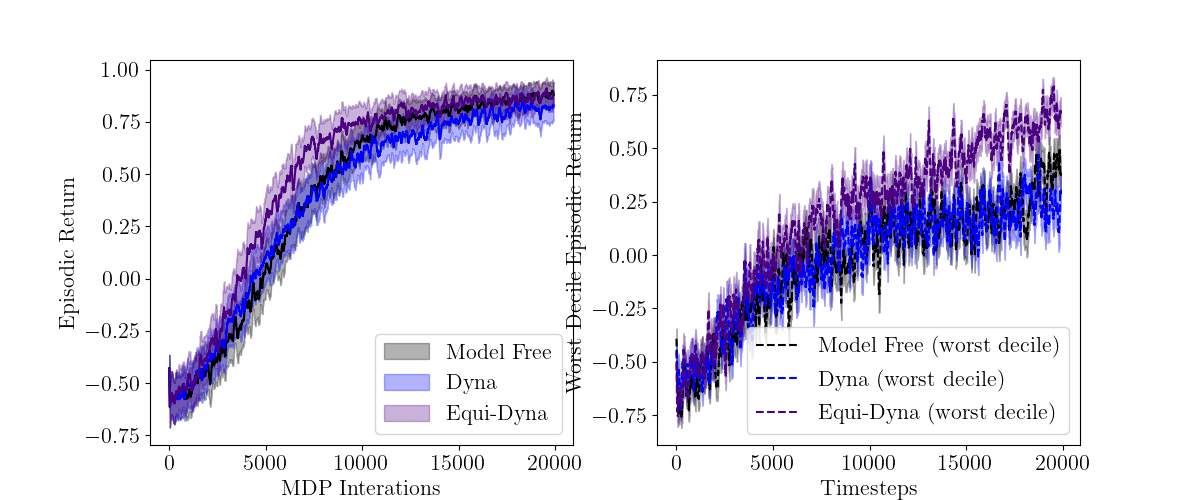
\includegraphics[width=\textwidth]{Figures/Expert_Dyna_Catch_pr2.png}
	\caption{Left: Mean episodic returns for the Catch agents across 128 random seeds
		plotted against number of interaction time-steps in the MDP. Right: The mean
		cumulative episodic returns of the worst performing 128 random seeds against
		number of experience time-steps in the MDP. Both of the plots are moving
		averages, with windows of 10 time-steps. Additionally, two standard errors are
		plotted. A planning ratio of 8 is used for equi-dyna and 4 for dyna.}
	\label{fig:supervised-dyna-catch}
\end{figure}

Inspecting the returns in Fig.\ref{fig:supervised-dyna-catch} we see that the equivariant transition model agent (equi-dyna) slightly outperforms the dyna model. The performance delta is most notable early on in the training. This is despite both of the transition models achieving near perfect accuracy on the validation dataset. Notably, though the worst decile of random seeds do perform better across both of the model based agents. In the case where the equivariant transition model, and the conventional MLP have the same validation error. One would expect that their ability to plan trajectories would be approximately equivalent. This does seem to be the case. However, the quality of the models seems insufficient to be a high quality substitute for actual transitions.

Again tabulating the returns' mean distribution in Table.\ref{tab:supervised-dyna-catch}. In the table only the best planning ratios are listed. This enables comparison with the G-CNN actor-critic, which vastly outperforms all dyna agents. Additionally, the distributions of the means are all within two standard errors for $50 \%$ and full sample completion.

\begin{table}
	\centering
	\begin{tabular}{|c|c|c|c|}
		\hline
		Time-steps & Baseline         & Dyna             & Equi-Dyna                 \\
		\hline
		$2, 000$   & $- 0.51\pm 0.07$ & $-0.41 \pm 0.09$ & $\mathbf{-0.29\pm 0.09}$  \\
		$10, 000$  & $0.70 \pm 0.06$  & $0.64\pm 0.06 $  & $\mathbf{0.67 \pm 0.05} $ \\
		$20,000$   & $0.875 \pm 0.04$ & $0.88\pm 0.06$   & $\mathbf{0.90\pm 0.05}$   \\
		\hline
	\end{tabular}
	\caption{Mean cumulative episodic returns tabulated for the two network architectures. All episodic returns are recorded with confidence intervals of two standard errors across 128 random seeds.}
	\label{tab:supervised-dyna-catch}
\end{table}

\subsection{Conclusion}
For both Catch and CartPole, the equivariant G-CNN transition models with a proximal pooling layer are capable of matching and/or surpassing the performance of the MLP transition models. Additionally, there is ample evidence to suggest that, when combined with the correct distance metric, the proximal pooling layer is sufficient to produce approximately equivariant transition models. This evidence is apparent in both Catch and CartPole, where a notable improvement in accuracy or reduction in loss on unseen data is observed. The G-CNN's ability to generalize to states not encountered in the training data is particularly significant if these states fall within the orbit of states seen during training.
When using the aforementioned transition models for performing supervised-dyna, mixed results were obtained. In the context of CartPole, the equivariant model's generalization improved significantly, allowing the agent to effectively utilize the planning phase and markedly enhance its sample efficiency. As a result, the agent required far fewer MDP time-steps to learn an expert policy

In the Catch environment, both the MLP and G-CNN models achieved identical accuracy after training. When employed to plan trajectories for a dyna agent, these models resulted in a slight improvement in the initial episodes compared to a model-free implementation. Furthermore, they exhibited significantly improved stability across the worst-performing random seeds.

The results of the supervised-dyna experiments indeed demonstrate the effectiveness of the dyna implementation. In certain scenarios, the transition model can effectively enhance an agent's sample efficiency. However, the marginal improvement in performance gained from models that generalize slightly worse suggests that the quality of the model plays a pivotal role in enabling effective model-based reinforcement learning. This observation is not surprising.
